\documentclass[../sablona-main.tex]{subfiles}

\begin{document}
	\section{Řešení úlohy za pomoci softwaru Excel}
	
	
	Tož nasázeli jsme do tabulky čísla:
	\begin{figure}[H]
		\centering
		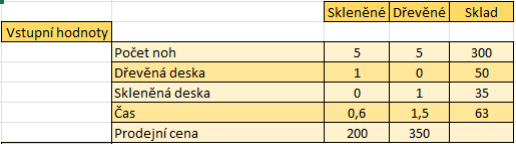
\includegraphics[width=0.7\linewidth]{kapitola5_0}
		\caption{Zadání údajů}
		\label{fig:kapitola50}
	\end{figure}
	
	Přidali jsme součty jednotlivých položek:
	\begin{figure}[H]
		\centering
		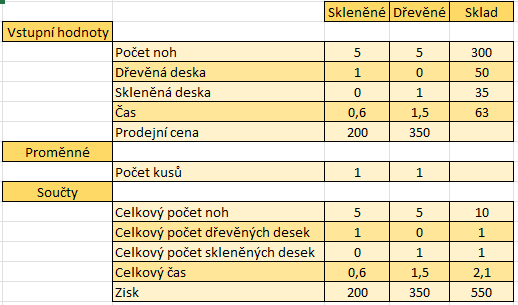
\includegraphics[width=0.7\linewidth]{kapitola5_1}
		\caption{Přidání součtů}
		\label{fig:kapitola51}
	\end{figure}
	
	Otevřeme řešitel a nastavíme podmínky:
	\begin{figure}[H]
		\centering
		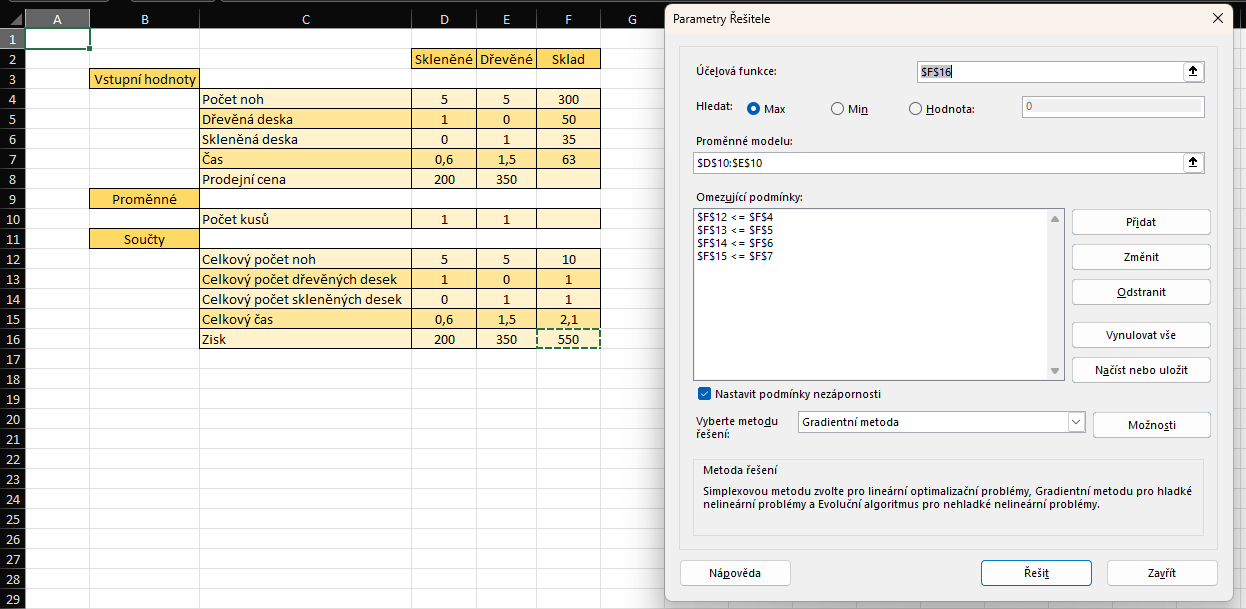
\includegraphics[width=0.7\linewidth]{kapitola5_2}
		\caption{Podmínky řešitele}
		\label{fig:kapitola52}
	\end{figure}
	
	Vyřešením získáme odpovědi:
	\begin{figure}[H]
		\centering
		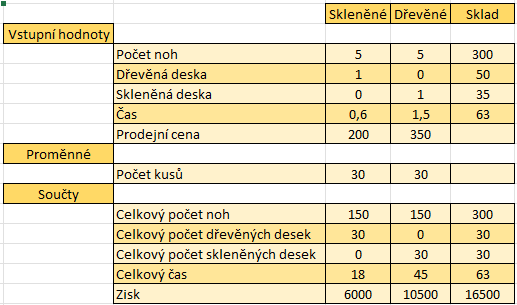
\includegraphics[width=0.7\linewidth]{kapitola5_3}
		\caption{Vyřešeno}
		\label{fig:kapitola53}
	\end{figure}
	
	Tedy optimálním řešením je vyrobit 30 dřevěných a 30 skleněných stolů se ziskem \$16~500.
	
\end{document}